%market

\subsection{Legislation}
Public perception that a TBTF policy exists creates distortions in an otherwise free market. 'Implicit backing' by the government can give favored financial firms merger premium advantages, bond funding advantages, liquidity advantages, and can exacerbate the 'too big' problem by enticing even more firms into their already swollen ranks.\cite{Baker}\cite{Brewer}\cite{Strongin}\cite{Rime} Oftentimes it is not sufficient for the government to remain passive during times of prosperity, they must actively deny holding a TBTF policy and even legislate directly against it. The first piece of major legislation targeting TBTF was passed in 1991 with the Federal Deposit Insurance Corporation Act (FDICIA) in response to criticisms that began after the government mishandling of the failure of Continental Illinois Bank in 1984.\cite{Wall}

The seventh largest bank in the US at its peak, it had made many imprudent business loans, especially to oil and gas companies hurt when energy prices declined, and overpaid for some acquisitions including Penn Square Bank which had made even more imprudent loans. It was also badly exposed in several developing markets where it had made some incorrect assumptions about future interest rates. As a result, the government needed to step in and acquire the failing institution. Fortunately, the bank did not have a large number of insured deposits; it funded itself in large part by taking brokered deposits too large to be covered by FDIC insurance, and by issuing notes and bonds.\cite{Peterson}

The government would traditionally opt for the entire firm to be liquidated unless a willing private sector acquirer could be found and asset values somewhat preserved in a buyout; instead of bank failure and liquidation.  However, on two occasions prior to the failure of Continental Illinois the FDIC had supported a failed bank by guaranteeing all creditors; not just the insured depositors.  In a widely criticized misstep, the government bailed out Continental Illinois. By the end of the situation the federal government had spent seven years and approximately \$1.1 billion to resolve Continental Illinois, with very little of the bank asset values preserved.\cite{Peterson}

An immediate liquidation would have been costless to the FDIC; Continental Illinois's assets would have managed covering the insured deposits, but later estimates suggest that six banks would have collapsed as a result; TBTF discussions began. The phrase had been used before, but became a household term after Congressman Steward McKinney charged that the FDIC had guaranteed uninsured deposits and bonds because it thought that Continental Illinois was 'too big to fail'. The FDIC denied the charge, claiming they were rightly acting to minimize taxpayer losses.

The FDIC continued to guarantee all creditors following this incident; uninsured depositors took losses in just 20\% of bank failures in the years leading up to FDICIA.\cite{Peterson} Before the Act, the indication to the public was that the economy was operating with a too big to fail policy in place, creating a dilemma for bank regulatory agencies.  Recall figure \ref{fig:div}, and subfigure \ref{fig:multiple}, that shows the expansion of investment to time-sensitive securities in the period leading up to the bailout of Continental Illinois in 1984.  This trend is larger than business cycle recessions, and pertains explicitly to the rise and fall of TBTF as it pertains to financial firms.

\begin{figure}[H]
\centering
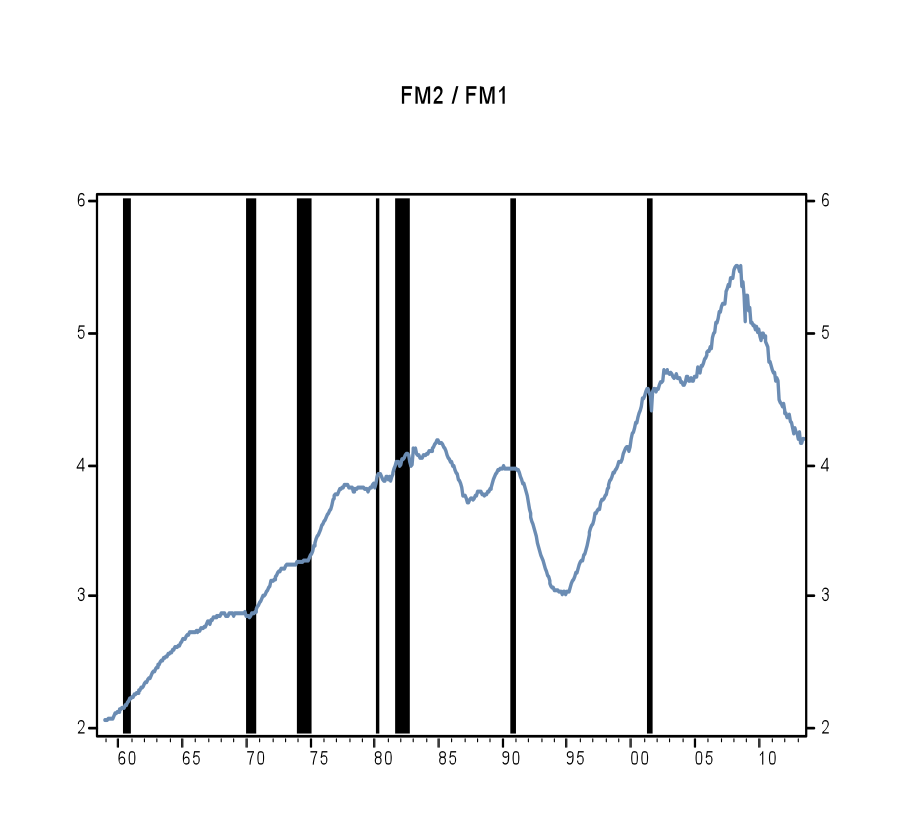
\includegraphics[scale=.70]{figure/HistoricalFM.png}\\[-0.7cm]
\caption*{M2 Divided by M1: Historic Leverage \label{no1}}
\end{figure}

FDICIA was passed with the intention of reducing taxpayers exposure to financial system losses, including their exposure at too big to fail financial institutions. By passing FDICIA, Congress was signaling that it was serious about ending 100 percent de facto deposit insurance.\cite{Wall} The FDIC had previously extending this guarantee after completing a process of comparing bids to acquire the entire bank (including all its deposits) with the cost of liquidating the bank, which generally produced the result that covering all deposits was less expensive. FDICIA sought to change this process by mandating least-cost resolution, which required consideration of all possible resolution methods. This mandate was widely understood as indicating that the FDIC should also consider purchase and assumption transactions in which the acquirer assumed only the insured deposits.

It is clear from the FDICIA measures to address specific systemic issues that the intent of Congress was virtually to eliminate the practice of TBTF. Although FDICIA did not ban the TBTF financial firm doctrine, it substantially reduced the likelihood of future large financial firm bailouts. Bankers and bank depositors could no longer casually assume that any given bank would be considered TBTF, and regulators became more likely to look for ways to close a large failing bank without protecting uninsured creditors. If conditions were such that a large fraction of the banking system was potentially not viable, regulators may have no choice but to protect uninsured depositors. However, for most other systemic risk situations, including financial market risk, the potential was created for identifying and developing alternate solutions.\cite{Wall} Indeed, the percentage of uninsured depositors who took losses in bank failures following the act and leading up to the 2001 crisis increased to 65\%, although this contrast is partially due to calmer markets than the decade previous had experienced due to the Savings and Loan Crisis.\cite{Peterson}\cite{Wall}

The final say on TBTF, the FDICIA, was eventually watered down in response to demands from regulators and the Bush administration that the FDICIA provide for a systemic exception to its requirement that problem financial firms must be resolved at the lowest cost to the insurance funds.  In the United States, the regulators wanted the right to deviate from the least cost resolution principle in the case of failure of an 'essential' financial firm.\cite{Kaufman}\cite{Rime}

Several years later the consequences of allowing Lehman Brothers to fail led the government to move aggressively to convince financial markets that they would not allow another major bank to fail in this manner. Congress passed the Troubled Asset Relief Program (TARP) to funnel hundreds of billions of dollars to support financial firms in a period of extraordinary financial turbulence. In addition, the Federal Reserve Board lent hundreds of billions of dollars to financial firms through a series of newly created special lending facilities. On top of these measures, the Federal Reserve and Treasury also took extraordinary actions to keep Citigroup and Bank of America solvent, at a time when they almost certainly would have collapsed without government support.\cite{Baker}

These circumstances led to the second major legislation effort against TBTF. In July 2010, Congress passed and President Obama signed the Dodd-Frank Wall Street Reform and Consumer Protection Act. Dodd-Frank's preamble states that one of the statute's primary purposes is to end TBTF and to protect the American taxpayer by ending bailouts. As he signed Dodd-Frank, President Obama declared, "Because of this law, . . . there will be no more taxpayer-funded bailouts. Period.''\cite{Frank}\cite{Wilmarth1} Dodd-Frank made meaningful improvements in the regulation of large financial firms.  It established a new umbrella oversight body named the Financial Stability Oversight Council (FSOC) that designates systemically important financial institutions (SIFIs) and makes recommendations for their supervision. Dodd-Frank also empowers the Federal Reserve Bank to adopt stronger capital requirements and other enhanced prudential standards for SIFIs. Most importantly, Dodd-Frank established a new systemic resolution regime named the Orderly Liquidation Authority (OLA), which aims to provide a superior alternative to the bailout or bankruptcy choice that federal regulators confronted when they dealt with failing SIFIs during the financial crisis.\cite{Wilmarth1}

Nevertheless, Dodd-Frank arguably did not solve the TBTF problem. Dodd-Frank relies primarily capital-based regulation, the same supervisory tool that failed to prevent the banking and thrift crises of the 1980s as well as the recent financial crisis. In addition, the supervisory reforms contained in Dodd-Frank depend for their effectiveness on the same federal regulatory agencies that failed to stop excessive risk taking by financial institutions during the booms that preceded both crises. Additionally, Dodd-Frank's most important reform for preventing future TBTF bailouts, the OLA, does not completely prohibit future rescues for creditors of large, complex financial institutions (LCFIs). The Federal Reserve Bank can provide emergency liquidity assistance to troubled LCFIs through the discount window and (perhaps) through 'broad-based' liquidity facilities that are designed to help targeted groups of the largest financial institutions.\cite{Wilmarth1}

While Dodd-Frank has undoubtedly made TBTF bailouts more difficult, the continued existence of these avenues for financial assistance indicates that Dodd-Frank is not likely to prevent future TBTF rescues during episodes of systemic financial distress and market leverage.  In effect, both attempts at strict regulation of TBTF instead became directives regarding the handling of a TBTF resolution regime.\cite{Kaufman}  Modifying the resolution regime assumes failure and is ex-post. It intended to reduce and reallocate the loss given failure. The remainder of this paper is focused on resolving insolvent large firms ex-ante.  We look to metrics that if controlled through policy, may reduce market volatility and extend financial stability. 

In choosing metrics to control it is important to realize that targeted legislation will always be vulnerable to the rapid evolution of financial firm practice.  Additionally it does not appear that the government is ever truly willing to deliver an ironclad regulation policy that eliminates TBTF once and for all in the face of potential systemic failure.  This ex-post stance is reasonable when considering that major financial firm assets are valued at nearer and nearer the per annum gross domestic product.

\subsection{Can Banking Get Worse?}

Despite these large and targeted attempts at regulation and prevention, bank crises are becoming decidedly more complicated and the bailouts larger in magnitude as a result of increasingly complex financial activities. Financial firms have grown into the role of profit generators who quite literally trade for their own benefit, ignoring the client investor, utilizing complex financial derivatives to generate large fractions of their income.\cite{Dowd} Accounting rules enforced by legislation such as FDICIA and Dodd-Frank have rapidly expanded as financial firm assets and liabilities have become more complex. However, financiers working together with lawyers and accountants have increasingly found ways around the intentions of regulators while remaining true to the 'letter of the law.'  

The regulator rules have grown more detailed and filled with technical jargon, but still fail to cover every possible circumstance of bad-practice investing; complex leverage positions. The rules have had the unfortunate effect of allowing financial firms to obscure true asset value from the growing pool of average wealth investors. It has become increasingly difficult to gauge the risk and value of the bank's portfolio. This has become a problem not only in financial derivatives and trading, but in areas of basic finance such as mortgage lending. 

Both professional and personal investors have begun to see large financial firms as 'black boxes,' and have no interest in investing in their stocks. This crisis of trust calls into serious question these complex practices whose failure could once again place the growth funds, pensions, or retirement funds of ordinary taxpayers in danger.

\subsection{Is There an Explicit Government Guarantee?}
 
While FDICIA attempted to make it more difficult for the Federal Deposit Insurance Corporation (FDIC) to protect uninsured depositors and creditors at large failing banking organizations and TBTF banking organizations, it is evident that a TBTF doctrine still exists. In fact, one might argue that FDICIA has actually formalized the process for bailing out TBTF banking organizations by specifically allowing a TBTF bailout when the banking organization's failure is deemed to have serious adverse effects on economic conditions or financial stability.  The formal approval process involves a two-thirds vote by the FDIC Board, two-thirds vote by the Federal Reserve Board, approval of the Secretary of the Treasury, and approval of the President of the United States.\cite{Brewer}  With this formalized process, "TBTF is now virtually official policy.'' \cite{Baker}

In the United States, both the Federal Deposit Insurance Corporation Improvement Act (FDICIA) in 1991 and the Dodd-Frank Act (DFA) in 2010 promised to limit, if not outright eliminate, TBTF in the financial industry.  This intent is made clear in the full title of the DFA, "An Act to promote the financial stability of the United States by improving accountability and transparency in the financial system, to end TBTF, to protect the American taxpayer by ending bailouts, to protect consumers from abusive financial services practices, and for other purposes...The language in the DFA remains evasive and leads to considerable confusion about whether TBTF has been effectively outlawed or institutionalized in the United States."\cite{Kaufman}

After Lehman's failure, Congress passed the Troubled Asset Relief Program (TARP) to funnel hundreds of billions of dollars to support financial firms in a period of extraordinary financial turbulence. In addition, the Federal Reserve Board lent hundreds of billions of dollars to the financial firms through a series of newly created special lending facilities.\cite{Baker}  It seems that the only consistent third party with enough liquidity to buy distressed financial firm assets is the government.  The government also maintains through its actions this tendency towards protecting the average American's wealth from the financial services they themselves choose to employ.  The government's frequency to act in financial recession, and the increased magnitude of that action is evident in this trend that started in the early 20th century with the Great Depression and the FDIC.  The government has built up the reputation that in times of hardship it must step in to protect the wealth of the nation.

In an ex-ante perspective, regulators and the government must diagnose the broad market investing trends that have led to financial firm bailout periods.  The regulator and government role should be heavily focussed on pinpointing precarious asset valuation, because leverage in finance can disastrously mix with faulty asset pricing to cause a market wide devaluation process.  The government and the american taxpayer continue to be called upon to purchase devalued illiquid assets.  Systemic problems are tied to distorted asset prices being used to leverage ever further.  


